%!TEX root = ../report.tex

%%%%%%%%%%%%%%%%%%%%%%%%%%%%%%%%%%%%%%%%%%%%%%%%%%%%%%%%%%%%%%%%%%%%%%%
\chapter{Arbejdsmarkedets opdeling: Segmenteringsteori. \label{segteoriteori}}
%%%%%%%%%%%%%%%%%%%%%%%%%%%%%%%%%%%%%%%%%%%%%%%%%%%%%%%%%%%%%%%%%%%%%%%

\vspace{20pt} \epigraphfontsize{\small\itshape}
\epigraphfontsize{\small\itshape}
\epigraph{“Labor markets constitute a means of mediation; they reflect the underlying forces in the production and in the laboring population.”}{--- \textup{\parencite[177]{Edwards1979}}}


Arbejdsmarkedssegmenteringsteorien opstod historisk som en kritik af og et alternativ til den nyklassicistiske økonomiske skole, hvori arbejdsmarkedet og agenterne på det behandles stort set som et hvilket som helst andet varemarked. Kernen i denne kritik er en forståelse af individerne på arbejdsmarkedet som drevet ikke af nyttemaksimerende økonomiske motiver, men bestemt gennem de sociale relationer og institutioner, individerne er indspundet i \parencite[173]{Boje1986}. Jeg vil i det følgende kalde det segmenteringsteori\emph{erne}, da der er tale om teorier med nogle fælles basale antagelser, der dog udmønter sig i vidt forskellige teorier om arbejdsmarkedets funktionsmåder \parencite[177]{Edwards1979}. 

% Denne afhandling vil tage udgangspunkt i segmenteringsteorierns grundlæggende forståelse af  arbejdsmarkedet og individerne på det, og kun sjældent forholde sig til den neoklassicistiske økonomiske skole. For en kritisk gennemgang af denne skole, med særligt fokus på dennes forståelse af arbejdsløshed, kan man læse Gravholt-Nielsens (2016) afhandling. 

Arbejdsmarkedets funktionsmåde og beskæftigelsespositioner på arbejdsmarkedet er i disse teorier forstået som "\emph{(...) den vigtigste institution, hvorigennem social ulighed og sociale konflikter om fordelingen af samfundets materielle og immaterielle goder opstår og afgøres}" \parencite[10]{Boje1985}. 
% Selvom denne forståelse indenfor sociologien har været kritiseret de sidste femoogtyve år \parencite[23]{Scott2000}, er det udgangspunktet for denne afhandling, at segmenteringsteorien og klasseteorier har ret i denne grundantagelse, om end det anerkendes at betydningen af position på arbejdsmarkedet, særligt i forbrugsvaner og individernes selvforståelse, har ændret sig markant i løbet af det tyvende århundrede. 
En central forskel fra den neoklassiske skole, er at arbejdsmarkedets heterogenitet og arbejdsstyrkens inhomogenitet er udtryk for grundlæggende sociale strukturer, der fortjener en plads som sådan i teoridannelsen. I den neoklassiske skole antager man markedsmekanismerne som \emph{i princippet} den mest effektive måde at allokere arbejdskraft på arbejsmarkedet, og barrierer for denne allokering skal findes i imperfekt information på markedet, stivhed i løndannelsen ud fra bestemte (blah blah skriv senere og find henvisning senere. Søren viste mig den der økonomiske grundbog hvor der stod at fagforeninger var en barriere fordi det hindrede den nødvendige frie løndannelse der sikrer effektiv allokering, kan måske bruges)

Arbejdsmarkedet opfattes i segmenteringsteorierne som bestemt ud fra samfundets struktur og organisering, det vil sige forholdene i produktionen af varer, de institutioner og deres normer, der er opstået som følge af historiske konflikter, samt de forskellige sociale grupper, som arbejdsmarkedet udgøres af \parencite[9]{Boje1985}. Det  vil sige, at disse barierer, som forhindrer fri mobilitet på arbejdsmarkedet, ikke ses som barrierer for den fri allokering af arbejdskraft ud fra udbud/efterspørgsmekanismer i et i princippet perfekt marked. I stedet ses disse barrierer for mobilitet som udtryk for de grundlæggende sociale mekanismer, som arbejdsmarkedet, og i sidste instans samfundet, består af. Arbejdsmarkedet er, som Boje siger, derfor mere kendetegnet af opdeling end af fri konkurrence \parencite[8]{Boje1985}. 


(skal måske ikke være her, men god indledning til afsnittet)
Pioeringer og Doire beskriver også dual labour market, men ud fra en tankegang om den amerikanske økonomi som opdelt i en kerneøkonomi bestående af store stabile firmaer og en perifær økonomi bestående af små og omskiftelige firmaer (Averitt). Denne tankegang forekommer meget bundet til den amerikanske økonomi, og muligvis også en bestemt periode. GER beskæftiger sig med sammme opdeling, men fokuserer på et todelt arbejdsmarked ud fra andre perspektiver. Store dele af deres analyse i deres hovedværk divided labor, divided workers fra 1982 indeholder samme fokus på USA og amerikanske forhold er et ringe sammenligningsgrundlag ifht. det danske samfund. Men de benytter en analysemodel, som jeg mener er ganske nyttig til at forstå arbejdsmarkedets relation til andre dele af økonomien og klassestruktureren generelt, og som giver nogle redskaber til at forstå segmenteringsprocessen. Redskaber jeg vil benytte mig af i min efterfølgende empiriske analyse af det det danske arbejdsmarked og sammenhængen til klassestrukturen. 



\section{det todelte arbejdsmarked \label{GER}} 

teorien om det todelte arbejdsmarked, ser arbejdsmarkedet som delt i to submarkeder, eller segmenter, et primært og et sekundært. Denne segmenteringsteori blev udviklet som kritik af den nyklassiske skole, for at begribe en udvikling i USA i 60'erne, hvor fokus på uddannelse og individuel frihed som vejen til at løse sociale problemer og reducere fattigdom, havde vist sig langt mindre effektiv end antaget \parencites[63]{Leontaridi1998}[1231]{Cain1976}. 

%findes der ikke en retning indenfor økonomien der taler om center-perifæri økonomi? Hvad hed ham der skrev den der bog om det? Hvad pokker hed han?

Gordon, Edwards og Reich (GER) udvikler i deres udgave en marxistisk inspireret analyse af de historiske forhold, der har ledt til det todelte, segmenterede arbejdsmarked. Det spørgsmål, de stiller - som alle andre marxister efter 2. verdenskrig, kunne man tilføje - er, hvorfor kapitalismens transformering af en bred gruppe af befolkningen til en klasse af arbejdere, ikke endte med en opkomsten af en \emph{klasse-for-sig}, i denne proletariseingsproces.  De forkaster den traditionelle marxistiske analyse, som “\emph{(...) generate mechanical theories of historical inevitability in which the emergence of a class-conscious proletariat always lurks around the next corner}” \parencite[21]{Gordon1982}. I deres bog \emph{Divided Work, Divided Workers} (1982) benytter de en historisk kontingent analysemetode, inspirereret af bl.a Ernesto Laclau og Eric Olin Wright, der betoner den relative autonomi af politiske og ideologiske kræfter i samfundsudviklingen. GER laver en langsigtet historisk klasseanalyse af hvad de ser som tre perioder i den amerikanske kapitalisme, hvoraf det segmenterede arbejdsmarked er den seneste periode. Selvom analysen en konkret iagtagelse af den historiske udvikling af institutionelle forhold på det amerikanske arbejdsmarked, og amerikanske forhold der spiller ind på dette generelt, er analysemodellen, og dens syn på arbejdsmarkedet, brugbart for denne afhandling, med en række forbehold, der vil blive taget op når det er relevant. 

GER arbejdsmarkedet som et af de vigtigste områder, hvori gennem klassernes sammensætning og relative styrke bestemmes. De skriver:
%
\begin{quote} \small %\raggedright %(bloktekst on/off)
Here, employers and workers bargain over the effective wage rate, the hours of work, and other elements of the wage-labor contract. The outcome of this bargaining reflects an extraordinarily wide range of forces: the extent to which workers are unified or divided, the intervention of the state, the ability of capitalists to develop new wage-laboring populations, the availability of new labor-saving technologies, the elements of race and ethnicity, the pace of accumulation and hence the strength of the macroeconomy. Nothing the extent of the development of the five major dynamic tendencies of capitalist economies is not sufficient. \sourceatright{\parencite[21]{Gordon1982}}
\end{quote}
%
Dette skal ses som en vægtning af det de konkrete institutionelle forhold, med særligt fokus på arbejdsmarkedet, som relevant for at forstå økonomien og klassestrukturen i samfundet. I modsætning til en mere abstrakt analyse af de love eller tendenser, der typisk tillægges vægt i en marxistisk-politisk økonomisk analyse, og som GER benævner som de fem store dynamiske tendenser sidst i ovenstående citat: \label{kapitalakkumulation} 1) Kapitalens tendens til at udvide grænserne for det kapitalistiske system, 2) koncentrationen og kontrollen af kapitalen i færre hænder, 3) lønarbejdet udbredes som den dominerende produktionsmåde d4) ændringer af arbejdsprocessen gennem ny teknologi, nye maskiner, nye måder at lede arbejdet på, samt  5) arbejdernes kamp for at beholde eller udvide goder i forbindelse med kapitalens processer. %her kunne godt laves noget fancy med at det den første sætning i hver af de fem punkter blev med fed, eller sådan noget 
Det er GERs argument, at disse fem tendenser bedst forstås ikke abstrakt teoretisk, men indenfor hvad de kalder \emph{akkumulationens sociale struktur}. Denne sociale struktur defineres som det miljø, hvori det enkelte firma opererer og akkumulerer kapital%
%
\footnote{kapital og akkumulation af denne skal her forstås i marxistisk forstand: Ikke som penge, men som et socialt forhold: \emph{Capital is value in motion}, som David Harvey engang omtalte det som. Den sociale proces, hvori menneskers arbejdstid omsættes til ren bytteværdi, nemlig penge - Hvad Marx kaldte \emph{den universelle ækvivalent} (HENVISNING TIL KAPITALEN), der igen kan investeres i at arbejde, så mere bytteværdi kan udvindes gennem menneskeligt arbejde. Et socialt forhold, således forstået.}%
%
.

j I første fase af kapitalakkumulationen er samlingen af de nødvendige input i produktionsprocessesen. Dette inkluderer råvarer, halvfabrikata og arbejdskraft, hvoraf det sidste nævnes som den mest problematiske af de tre:  
%
\begin{quote} \small %\raggedright %(bloktekst on/off)
Labor supply, the most problematical of the three, involves both structure of the labor market, determining the immediate supply of labor, and the social institutions (family, schools, etc) that reproduce the labor force generationally\sourceatright{\parencite[24]{Gordon1982}} \label{aksocstruk}
\end{quote}
%
Efterspørgslen på arbejdskraft indeholder både arbejdsmarkedet, hvor den nødvendige arbejdskraft med de efterspurgte kompetencer købes på det påkrævne tidspunkt. Det indeholder dog også det langt større felt af sociale institutioner, der sørger for arbejdskraftens sammensætning og kompetenceniveau mere bredt forstået. Det vender jeg tilbage til.

% kunne godt referere til Fligstein her måske

Anden fase af kapitalakkumulationen foregår indenfor firmaet selv. Det indeholder organisering af selve arbejdsprocessen og management-strukturen i firmaet. Den fase kan siges ikke at have så meget med miljøet at gøre som med firmaets interne organisering. GER påpeger at det, der her tilsigtes, er de normer og erfaringer for organisering og management, som firmaerne trækker på, og som derfor er en del af den sociale struktur, det enkelte firma trækker på i dets akkumulationsproces. Denne organisering af arbejdet og ledelsen af arbejdet er central for eksempelvis fagforeningernes betingelser for at organisering. Det har også - lidt mere diffust men ikke mindre vigtigt - vidtrækkende konsekvenser for de livserfaringer, det enkelte menneske gør sig, og dermed hvordan det fortolker verden omkring sig. (REFERENCEMÅSKE?). 

Den tredje fase er salgsprocessen, hvori vareefterspørgsel,  samt status for konkurrencetilstande på det specifikke marked, et givent firma producerer til. Det kunne eksempelvis en være monopollignende tilstand, hvilket muliggør en bestemt virksomhedsstruktur. 

Det er særligt første og anden fase, der har min interesse, da det jeg er interesseret i er arbejdsmarkedet og dets relation til klassestrukturen. Tredje fase har dog en meget vigtig mekanisme i relation til arbejdsmarkedets segmentering, ifølge GER, som bør fremhæves, og som leder over i GERs teori om det todelte arbejdsmarked og forklaringen på denne.

Konkurrencetilstanden på markedet har betydning for arbejdsmarkedet generelt, ikke bare af den åbenlyse grund, at det skaber den økonomiske virkelighed for de virksomheder, lønmodtagerne er ansat i. Konkurrencetilstanden på markedet er også en af de væsentligste forudsætninger i GERs segmenteringsteori om et todelt arbejdsmarked. De viser hvordan man I USA fra 30'erne og frem udviklede store firmaer, med stabile profitrater og undertiden monopollignende markedsandele, såvel på hjemmemarkedet som internationalt. Disse firmaers størrelse og stabilitet gav mulighed for \emph{interne arbejdsmarkeder}, hvorigennem kompetencer kan udvikles internt, karrieremuligheder sikrer loyalitet, og andre fordele forbundet med hvad GER kalder \emph{bureaukratisk kontrol}. Dermed menes der management systemer, der kunne strukturerer og sikre størst mulig samarbejdsvillighed og produktivitet fra arbejderne i arbejdsprocessesen. Det er en af årsagerne til fremkomsten af interne arbejdsmarkeder i store firmaer, der af GER karakteriseres som det \emph{kernesegmentet/det primære segment} \parencite[187]{Gordon1982}. Det ville næppe være muligt for firmaer fungerende på usikre markeder med lav profitrate at skabe disse strukturer  

På denne måde kan vi se at de fem dynamiske tendenser nævnt på \ref{kapitalakkumulation} hænger sammen med den akkumulations sociale struktur, hvorigennem disse lovmæssigheder i en marxistisk optik fungerer. Den femte tendens er ikke med i ovenstående (korte) forklaring, og er centralt for at forstå segmentering generelt, og den amerikanske todeling specifikt. Det er arbejdernes modtræk, og ikke mindst arbejdsgivernes modtræk til disse modtræk, så at sige. 
Fagforeninger spiller naturligvis en væsentlig rolle i GERs analytiske perspektiv. Det er deres argument, at fagforeningers styrkeposition fra 30'erne og frem, også i USA, banede vejen for et klassekompromis, hvor arbejdsgiverne blev tvunget til at give indrømmelser omkring stabile ansættelser, reallønstigninger og sikre arbejdsforhold. En række krav blev imødekommet, og det er GERs pointe, at arbejdsgiverne til en vis grad var klar over nødvendigheden af dette. Den tidligere sociale akkumuleringsstruktur, som GER analyserer indgående og klassificerer som homogeniseringsperioden fra 1870 til slutningen af Anden Verdenskrig, mente man, gavnede radikale elementer i arbejderbevægelsen, og derfor var visse indrømmelser at foretrække. Der var desuden nok at gøre med at tilrettelægge arbejdsprocessen til ny teknologi og nye måder at styre, uddanne og inddele arbejdsstyrken på. Her kunne fagforeninger også bruges som samarbejdspartnere \parencite[186f]{Gordon1982}. Denne overgivelse af bureaukratisk magt attribuerer GER til tre hovedårsager, nemlig muligheden for reallønstigninger og en række sikringer af arbejdstagerrettigheder, hvilket muliggjordes af det økonomiske boom efter 2. Verdenskrig. De to andre faktorer var udrensning af radikale elementer i fagforeningerne i McCarthy-æraen, samt en mulig mangel på indsigt i konsekvenserne af den bureaukratiske kontrol, og hvad den betød for lønmodtagernes styrkeposition. Denne   

Logikken i det nye system, der derved blev udviklet, kan opsummeres på følgende vis: Jobs blev findelt i specifikke jobfunktioner, ofte indenfor trin i en karriertrappe. Ny teknologi påvirkede ikke kun hastigheden og arbejdskvaliteten, men blev også benyttet med det bredere formål at akkomodere managementpolitik, reguleringen af arbejdet og arbejderne som sådan. Ansættelser, forfremmelser og afskedigelser blev systematiseret og bureaukratiseret. Forhandlinger mellem arbejdergiver-fagforeninger blev i højere grad et spørgsmål om løn og frynsegoder, mens arbejdsforholdene og arbejdspladsens indretning blev til managementpolitik, udviklet af ingeniører og forløberne til HR-konsulenter. Det betyder at arbejdsmanagement skiftede karakter fra en intervention fra ledere eller mellemledere og deres direkte autoritet, til et spørgsmål om regulativer og procedurer \parencite[189]{Gordon1982}%
%
\footnote{Udviklingen af bureaukratisk autoritet er en tendens Max Weber beskriver så tidligt som i 20'erne. Man kan anskue det sådan, at GER viser hvorledes denne autoritetsform rodfæster sig i den samfundsmæssige produktion i årtierne efter, og at dens konkrete udformning og formål - udover at have sin egen indre logik, jvf. “rationalitetens jernbur” - sker på basis af magtkampe mellem klasserne. (FIND HENVISNING WEBER).}%
%
. 


Det er denne virksomhedsstruktur, der danner basis for det primære segment af arbejdstagere.

Det \emph{sekundære/perifære} segment består af job i små og mellemstore virksomheder, ofte ejet af et enkelt individ eller en familie, i begrænsede markedspositioner, tit med usikker eller stærkt variende efterspørgsmål. Profitten er typisk lavere end i kerneøkonomien%
%
\footnote{betegnelserne kerneøkonomi og den perifære økonomi er stammer fra den amerikanske økonom Robert Averitt, der i 60'erne benyttede denne betegnelse til at forstå den amerikanske økonomi, dog ikke ud fra det klasseperspektiv GER benytter i deres segmenteringsteori. Det her står vist også et andet sted \#todo}%
%
, og økonomiske kriser resulterer ofte i konkurs eller alvorlige finansielle problemer. Teknologi og marketing er sjældent up to date med firmaer i kerneøkonomien \parencite[7]{Averitt1968}. Det sekundære arbejdsmarked har som følge deraf lavere lønninger, større risiko for arbejdsløshed, mange midlertidige  stillinger og andre dårlige ansættelsesforhold \parencite[70f]{Doeringer1971}.

GER peger på at firmaer i den perifære økonomi tjener et formål, og der er grunde til at de ikke overtages af kernefirmaerne: Det er usikre markeder med svingende, ofte lavt, afkast. Det giver kernefirmaer mulighed for outsourcing af bestemte opgaver, der er billigere end indenfor de restriktioner, det primære beskæftigelsessegment muliggør. Særligt i forbindelse med varierende efterspørgsel: Det giver en fleksibilitet i at kunne hyre arbejdere fra det sekundære segment indirekte, gennem et sekundært firma, når efterspørgslen på et primærfirmas varer er høj, uden at være bundet op på forpligtigelser når efterspørgslen er lav \parencite[191]{Gordon1982}. 

Det primære uafhængige segment \label{GER kontrol og intern arb marked} indeholder de højere uddannede lønmodtagere indenfor professionerne, management og teknisk arbejde. De oplever et højere økonomisk afkast ved deres uddannelse%
% 
\footnote{GER skriver at de opnår “\emph{a higher return to schooling and experience}” \parencite[202]{Gordon1982}, hvilket jeg tolker som \emph{relativt} til det underordnede segment, det vil sige at de økonomisk får mere ud af x antal års uddannelse eller erfaring end en person beskæftiget i det underordnede segment.}%
%
, og der er sjældent en direkte supervision af og autoritetsudøvelse over udførslen af deres arbejde. De er desuden tilbøjelige til at internalisere firmaets formål. 
Historisk udspringer dette, ifølge GER, af proletariseringen og de deraf følgende konsekvenser af nogle traditionelle klasser i forbindelse med kapitalismens tidligere akkummulationsstruktur, i GERs jargon kaldet \emph{homogeniseringsperioden}.  Dette skete indenfor eksempelvis håndværkerlaug, samt andre med højtudviklede faglige ekspertiser. Ekspertise på de niveauer var i midlertidigt en nødvendighed, og en omkalfatring af disse traditionelle klasser ledte til fremkomsten af positioner i den primære økonomi, hvoraf formel uddannelse med tæt tilknytning til “arbejdsmarkedets behov”, altså arbejdsgivernes behov, fandt sted. Det skete naturligvis ikke uden klassekamp, så GER pointerer at disse erhvervsgruppers nuværende position også er et resultat af de modtræk, erhvervsgrupperne benyttede sig af, for at sikre sig autonomi og andre goder, eksempelvis ved oprettelsen af hvad GER kalder “professionelle associationer”, man kunne forestille sig at DJØF og IDA kunne eksempler i en dansk kontekst. Resultatet af denne torvtrækning med arbejdsgiverne, til en vis grad vellykket, betød følgelig skarpere segmentering ifht. det primære underordnede segment \parencite[202f]{Gordon1982}.
Dette kan også tolkes som GERs bud på hvad Eric Olin Wright kalder “the problem of the middle classes” i marxismen, altså hvilken historisk rolle og nuværende position, man skal forstå middelklasserne i, i en marxistisk optik. Mere om det i afsnit (??? \#todo).

Det “\emph{primære underlagte}” segment har ikke nødvendigvis udsigt til betydningsfulde forfremmelser, men er i stedet motiveret af stabil jobsituation og lønforhøjelser gennem anciennitet. Deres arbejdsprocess er superviseret og indeholder meget repetitivt, rutinepræget arbejde, med specifikke regler for dets udførsel og direkte autoritetsudøvelse i forbindelse med overholdelsen af disse. Der er ikke kun tale manuelt arbejde af den traditionelle arbejderklasse-forestilling, men også ikke-manuelt arbejde indenfor “\emph{white-collar}”jobs befinder sig i det primære underordnede segment (du må ku finde på en bedre beskrivelse \#todo) .  Disse er i langt højere grad organiseret sig gennem fagforeninger, da loyalitet til arbejdsgiverne ligger fjernere for beskæftigede i dette segment end i det primære uafhængige segment. \parencite[28f]{Drago1995} og \parencite[203]{Gordon1982}. (hvordan kan jeg få de her stå i samme parentes? \#todo).



Boje skelner mellem to former for segmentering: \emph{premarket} segmentering og \emph{inmarket} segmentering. Det er ganske simpelt forskellen på den stratifikation, der foregår på arbejdsmarkedet, og den, der finder sted før arbejdsmarkedet \parencite[46]{Boje1985}. At skelne disse fra hinanden i praksis er ikke nemt. Boje opstiller følgende model for forskellen mellem premarket og inmarket segmentering:
%
   \begin{figure}[H]
   \begin{centering}
   	\caption{Premarket og inmarket segmentering}
   	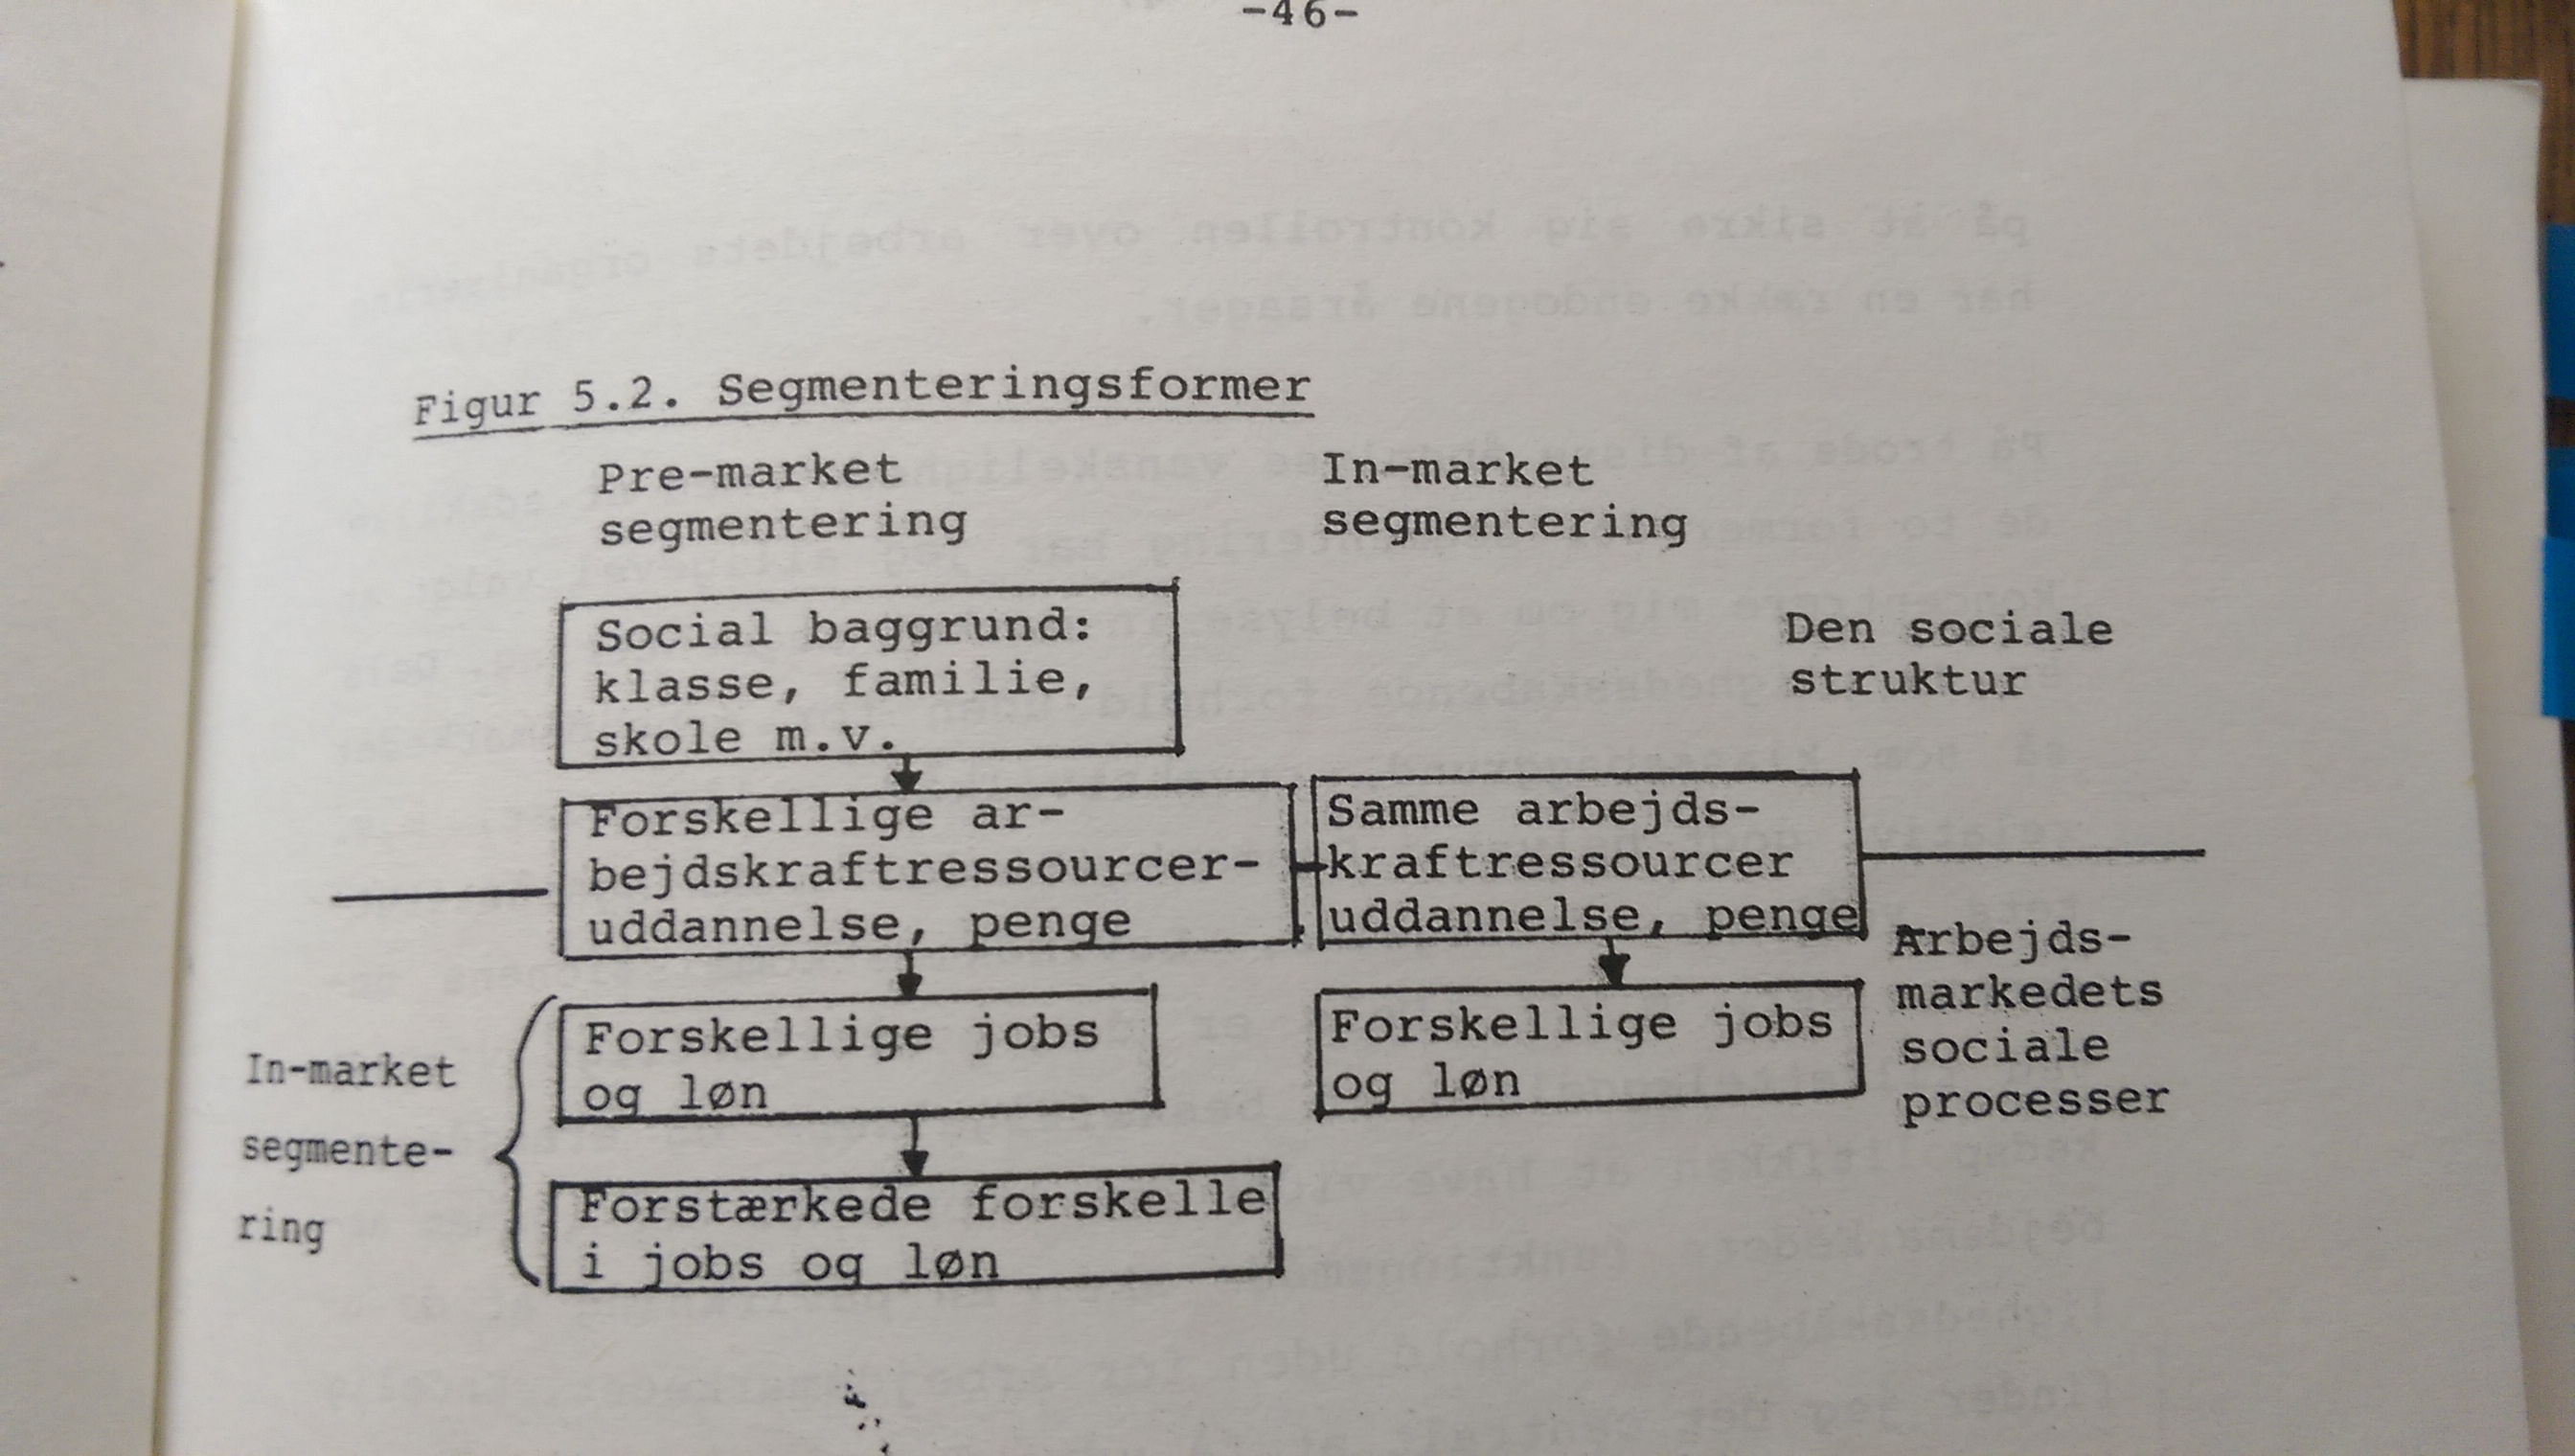
\includegraphics[width=\textwidth]{fig/Boje_premarket_inmarket.jpg}
   	\label{fig_premarketinmarket}
   \end{centering}
   \end{figure}   
%

Premarket segmentering ligger tæt op af hvad man kunne kalde den almene sociale stratifikation i samfundet, omend fokus er rettet på de stratifikationsformer, der bevirker at lønarbejdere stilles forskelligt ved indtræden på arbejdsmarkedet. 
Eksempelvis forskelle i kvalitet af uddannelsesinstitutionerne, familiens kulturelle og økonomiske ressourcer, samt  sociale netværk i forbindelse med eksempelvis skolekammerater og familiekontakt, der giver forskellige ressourcer ved indtrædelse på arbejdsmarkedet. 

Inmarket segmentering omhandler de mekanismer, der gør sig gældende på arbejdsmarkedet. Som Boje fremfører, er det dette, som GER bruger mest i deres forklaringsmodel \parencite[46]{Boje1985}.  (vend tilbage til det her, vurder hvilke eksempler der skal med. fx race, køn \#todo).

Det kan være svært at skelne disse to fra hinanden, og distinktionen er i mange sammenhænge en analytisk skelnen. I en dansk kontekst konkluderer Andrade, i en registerdata-baseret undersøgelse af nabolagseffekter på indkomst i perioden 1986-1988 og 2006-2008: “\emph{Although changes in the labour market appear to be the primary factor in the explanation of the reproduction of poor and wealthy neighborhoods, geographical movements can be viewed as a spill-over-effect in which individuals who no longer fit the socioeconomic profile of the neighborhood moves out of the the neighborhoods. These selection processses of geographical mobility in and out of neighborhoods have an active role in changing the neighborhood enviroment.}” \parencite[134]{Andrade2014}. Det vil sige, at selv det (kultur)geografiske landskab er påvirket af arbejdsmarkedets sammensætning - arbejdsmarkedet virker tilbage på premarket segmenteringen, der igen påvirker inmarket segmenteringen. 

Derfor kan det \emph{analytisk} give mening at skelne mellem sociale processer, der foregår direkte på arbejdsmarkedet, og de processer, der er en del af hele klassestrukturen. Det er inkorporeret i følgende udvikling af ASS-modellen, nu kaldet B-ASS (for Boje): 
%
\begin{figure}[H]
\begin{centering}
	\caption{B-ASS modellen}
	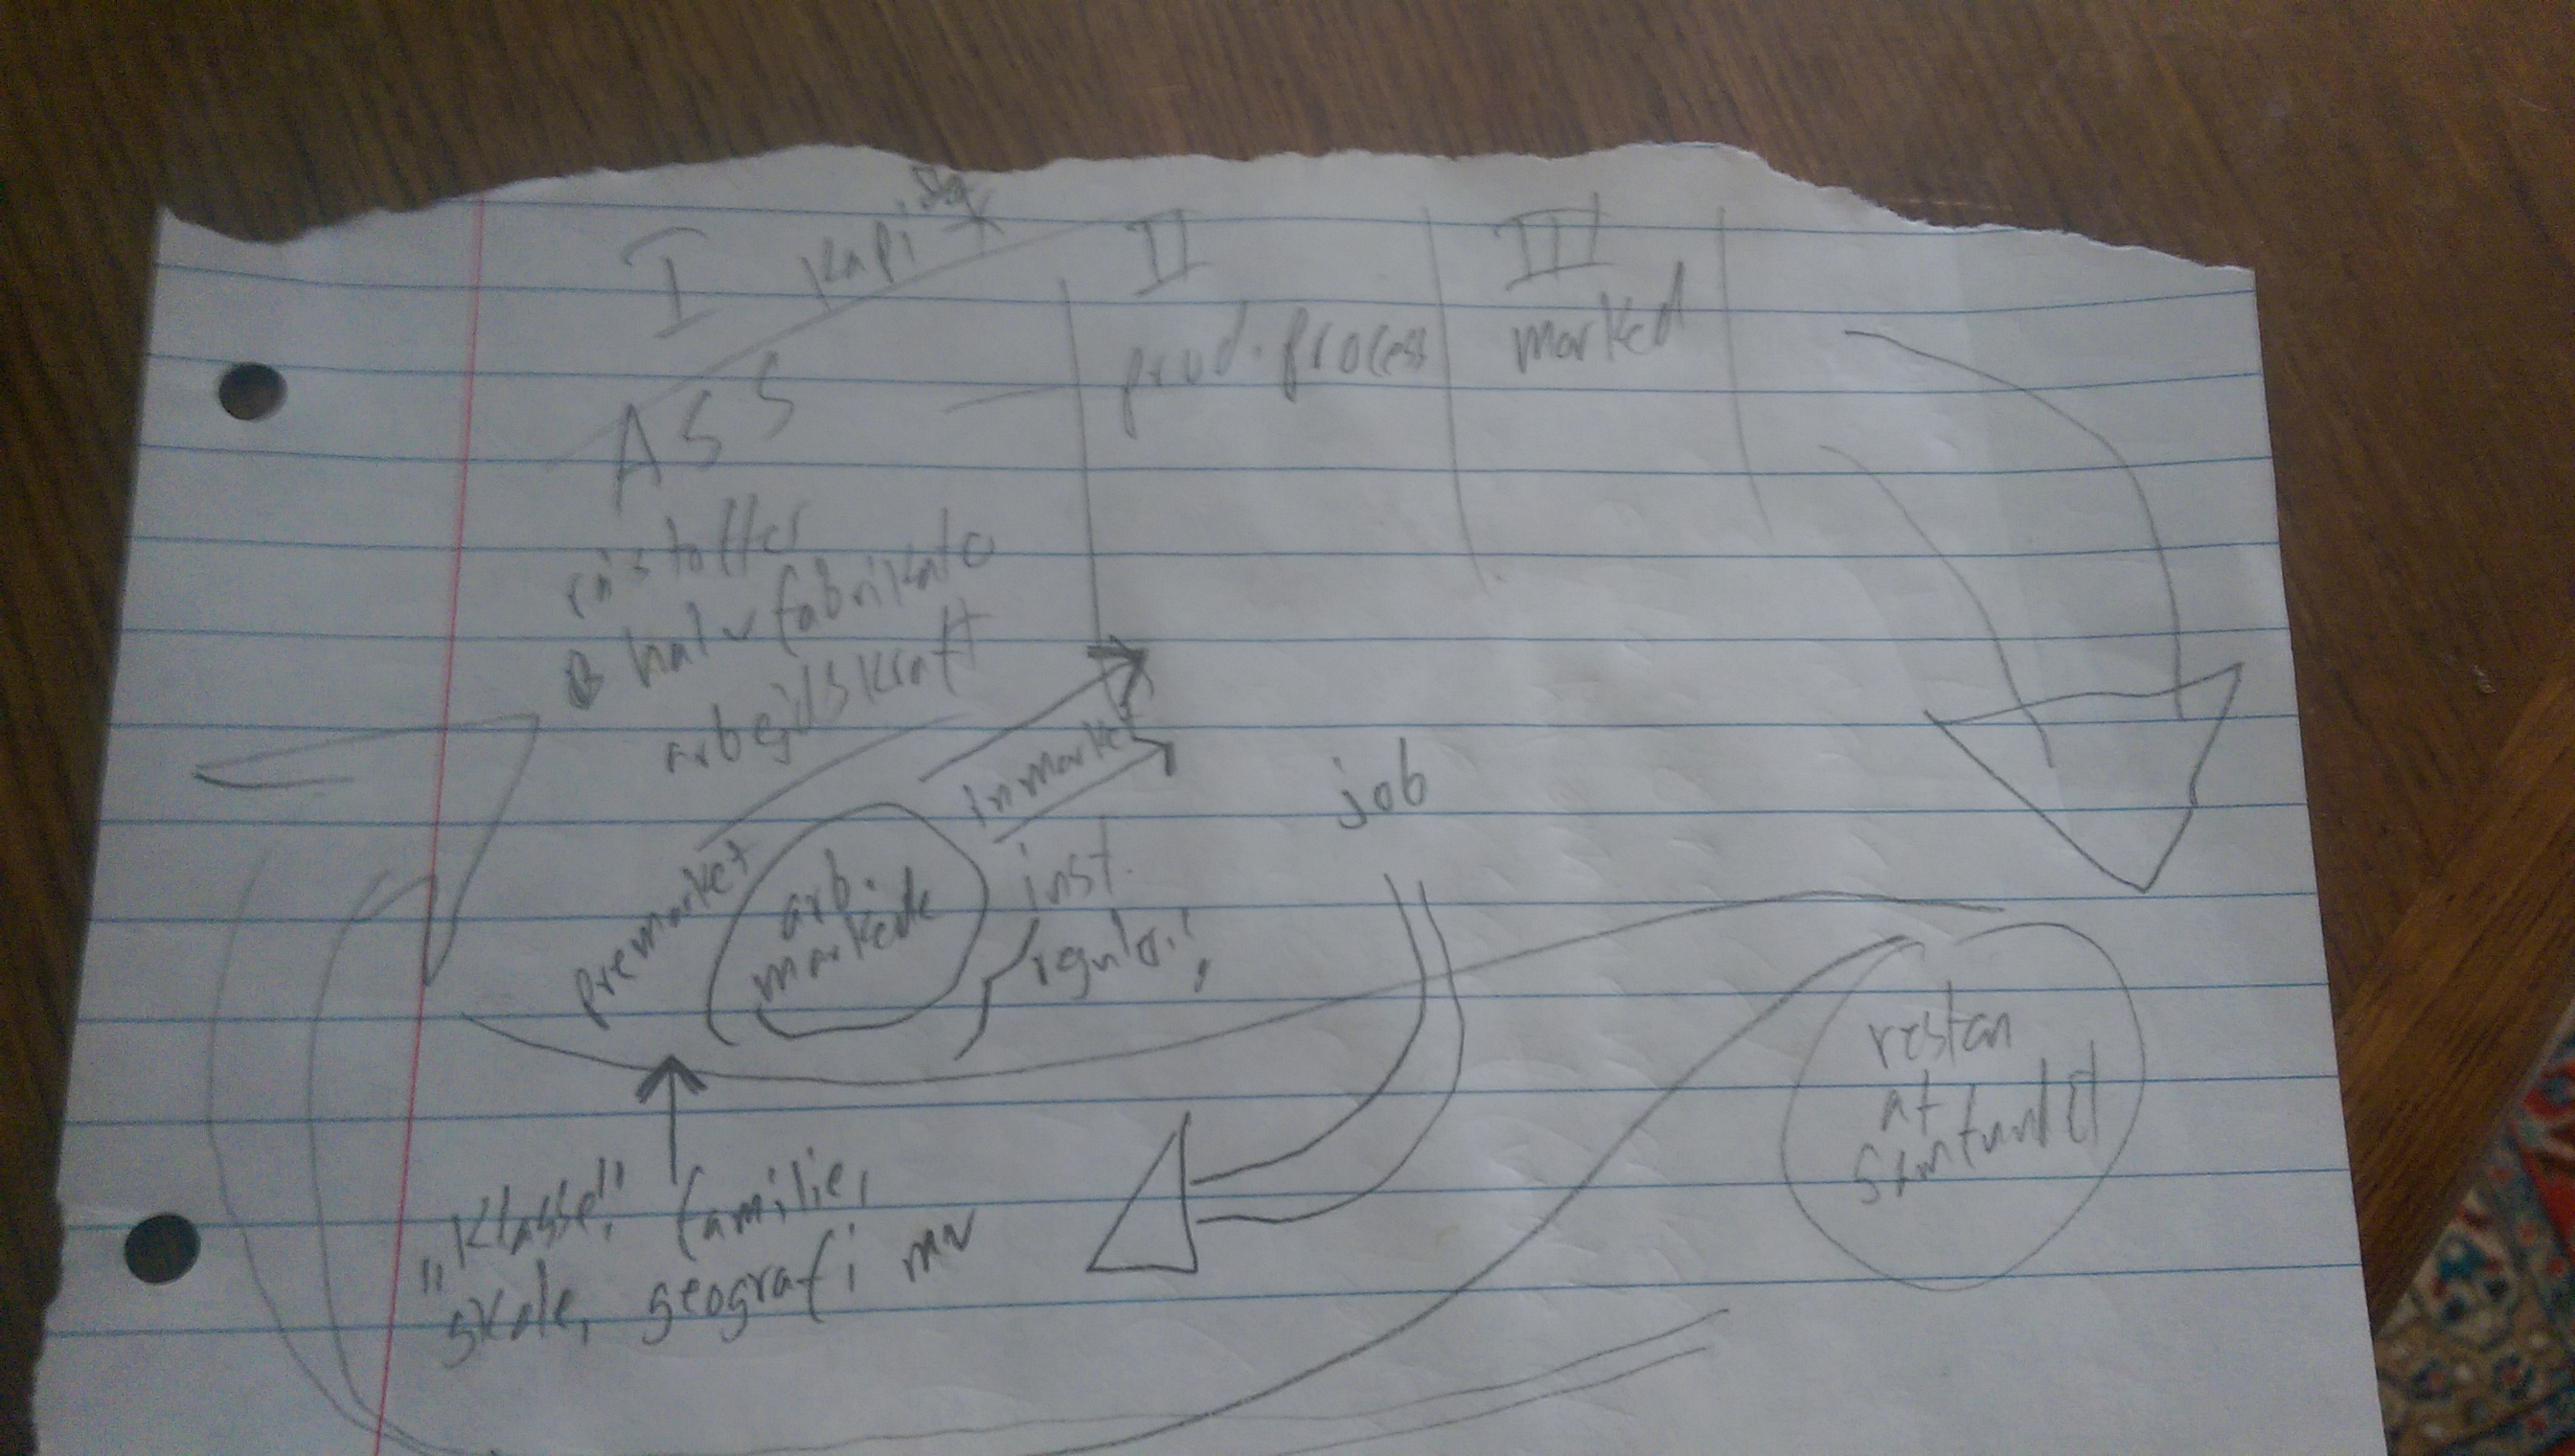
\includegraphics[width=\textwidth]{fig/B-ASS-model.jpg}
	\label{fig_B-ASSmodel}
\end{centering}
\end{figure}
%


GERs historiske redegørelse for klasseudviklingen i USA er, naturligvis, netop dette: en redegørelse for klasseudviklingen \emph{i USA}. Det betyder at en lang række af de sociale forhold, der gør sig gældende, ikke kan overføres til andre lande. Sammensætningen og betydningen af hvilke sociale strata, der findes, hvordan middelklassepositionerne er udformet, samt hvilke politiske alliancer, der findes. Det er centralt for udformingen af et samfund, som de siger, og fortsætter: “\emph{an emphasis on human agency rather than abstract laws in historical change, (...) the importance of historical contingency in shaping the responses of different groups to capitalist development, (...) and the diverse spatial and temporal paths of capitalist development.}” \parencite[21]{Gordon1982}. 

Det er derfor tankegangen og forståelsen af, hvorledes arbejdsmarkedet fungerer i klassestrukturen, der er brugbar i min afhandling. Denne vil jeg benytte i min egen analyse. 




Derudover har GERs teori samt empiri nogle problemer, der skal adresseres. Først de empiriske udfordringer samt bud på kortlægninger af segmenter, jeg har set på.

Det er en generel udfordring i segmenteringsteori, at der er meget lidt enighed om hvad der præcist karakteriserer et segment, hvordan segmenter er adskilt fra hinanden, og følgelig hvordan man empirisk observerer segmenter \parencite[71]{Leontaridi1998}, \parencite[1231]{Cain1976}. Følgelig er de indikatorerer og variable, der benyttes til at observere segmenter, vidt forskellige. Jeg vil her beskrive tre strategier, som jeg ser benyttet i litteraturen. Disse tre strategier benytter sig af forskellige variable, samt forskellige statistiske teknikker. 

Hvis man starter med GER, så er de overraskende nok utroligt vage i deres præcise beskrivelse af 

de benytter selv data på branche-niveau, men siger at brancher  indeholder både kerne- og perifæri firmaer. de mener med andre ord at data på firmaniveau er ideelt, men har ikke sådanne data til rådighed s. 193. De indikatorer, de benytter sig af, er primært mål for økonomisk formåen, hvori beviset for den 3-delte segmentering, de a priori har inddelt brancherne i, handler om den relative forskel mellem segmenterne, og særligt en stigende relativ forskel over tid. Det er indikatorer såsom værdi tilført per arbejder, lønforskelle per arbejder, andelen af produktionsjobs i forhold til total antal ansatte (indikerer antallet der er ansat indenfor management, salg, planlægning etc), samt faglig organisering. Alle disse sættes op relativt mellem GERs på forhånd inddelte 3-delte brancheopdeling \parencite[193]{Gordon1982}. Derudover kommer de med to interessante betragtninger om ting de \emph{ikke} har kunne måle: Udover at de helst ville have data på firma-niveauer, siger de også at indenfor firmaer i den primære økonomi, findes der sekundære og primære jobtyper. Derfor ville data på beskæftigelsesniveau fremfor firma- og branche være interessant, mener de \parencite[193]{Gordon1982}. 
Det andet de siger er de løb ind i problemer, da de skulle opdele ikke-manufaktor brancher i kerne-perifæri, da denne distinktion ikke let lader sig overføre udenfor den direkte materielle produktion af goder. Derfor er deres undersøgelse \emph{en undersøgelse af en tre-delt segmenteringsproces indenfor manufakturen i USA} \parencite[199]{Gordon1982}, mens segmentstrukturen andre steder i arbejdsmarkedet kan være anderledes indrettet, også i USA på det tidspunkt.

Man kan sammenfatte og sige at denne metode inddeler brancher efter en teoretisk styret logik baseret på et tre-delt arbejdsmarked, og benytter økonomiske nøgletal på brancheniveau som variable. Nøgletallene er antageligt populationsbaserede, fremfor survey-baseret (bliv sikker på det her senere \#todo) Herefter benyttes forskellene i nøgletallene mellem de tre teoretisk inddelte segmenter til at teste hypoteser om forskelle på segmenterne. De benyttede variable har et fokus på produktion og fagforeningsorganisering til at lave denne tredeling.  

Den anden strategi er benyttet i en australsk undersøgelse fra 1995, hvor Robert Drago (1995) finder at den tredelte segmentstruktur beskrevet af GER passer med det australske arbejdsmarked. Her benyttes survey-data på firma-niveau, og metoden er en  konfirmatorisk klusteranalyse. Det vil sige antallet af klustre er bestemt \emph{ex ante} til GERs tre segmenter, beskrevet i afsnit \ref{GER}. At observationsenheden er firmaer giver nogle problemer, bemærker Drago selv, da firmaer godt kan indeholde flere typer jobs, og her bliver de sat enten som uafhængig primær, underordnet primær eller sekundær. Variablene er andelen af manuelt arbejdende i forhold til ikke-manuelt arbejdende i firmaet, andelen af ansatte med jobancienittet på mindst 10 år, andelen af deltidsansatte, andelen af kvindelige ansatte, lønningsniveauer, andelen af supervisorer der er steget i graderne internt i firmaet og deslige. Drago finder at de tre klustre passer overordentligt godt med den tredelte segmentstruktur forudsagt af GERs segmenteringsteori \parencite[59]{Drago1995}. 

Man kan sige sammenfatte og sige at her er den empiriske test er noget mere avanceret, de segmentopdelingen ikke er lavet af forskerne selv, men i stedet bygget på en konfirmatorisk klusteranalyse, der baserer sine grupperinger på at minimere variansen indenfor det fastsatte antal klustre. Variablene er mindre fokuseret på økonomisk formåen i segmenterne og mere fokuseret på arbejdsmiljø. Og data er på firmaniveau. 

Gittleman og Howell (1995) benytter ligeles klusteranalyse deres undersøgelse af segmenter, men ud fra et andet udgangspunkt. De opsummerer segmenteringsteoretikernes empiriske forsøg på følgende vis: “\emph{the most common approach in empirical studies of segmentation, particularly when the unit of analyusis is occupations, has been to begin with the researcher's judgment about how many and what kind of rules to empirically implement the scheme, again based on the researcher's judgment. (...) the arbitrariness of this approach has been sharply critized.}” \parencite[422]{Gittleman1995}. Derfor benytter de i stedet en eksplorativ klusteranalyse, hvor antallet af segmenter ikke er defineret på forhånd. De benytter Wards hierarkisk-agglomerative klusterteknik. Det betyder at klustre merges sammen på stadig højere niveauer, sådan at to klustre, der merges på 2. niveau af klusterproceduren, hver især godt kan være sammenlægninger af tidligere klustre på 1. niveau, og så fremdeles, indtil visse varians-kriterier er opfyldt \parencite[425]{Gittleman1995}%
%
\footnote{
Man kunne måske forledes til at tro at de mener en udelukkende mekanisk inddeling er at foretrække, det er dog for simpelt. De når frem til 6 klustre, hvor de udelader en 7. kluster af teoretisk-praktiske grunde - de argumenterer for denne 7. gruppe er en undergruppe af et af de andre segmenter, da de sammenlagte jobtyper ikke adskiler sig væsentligt \emph{på et teoretisk niveau indenfor segmenteringsframeworket} fra den klynge, den kommer fra \parencite[424]{Gittleman1995}. Så der er mere tale om at lade empiri og teori spille sammen, hvor de mener det er problematisk at lade segmentinddeling være forhåndsbestemt.}%
%

De benyttede variable kommer fra en survey om arbejdskvalitet, og detaljerede informationer om respondernes beskæftigelse samt branche-tilhørsforhold. Gittleman og Howell benytter altså en kombination af jobs og branche for at kunne se forskel på \emph{samme} jobs indenfor \emph{forskellige} brancher. Og forskellige jobs indenfor samme branche, kunne man sige. 
Det er vigtigt at bemærke at denne at segmentopdelingen, ligesom hos Drago, baserer sig på en række mål for kvaliteten af jobs. Dette har naturligvis at gøre med en betragtning om at \emph{jobkvalitet}, og forskellene i disse, er definerende for hvad et segment er: Netop en social stratifikation, der giver bedre arbejdsbetingelser for visse grupper af mennesker i kraft af deres sociale position, da de herigennem - hvis man skal trække på GER - har mulighed for blah blah (skriv måske færdig senere men ikke engang sikkert det hører til her \#todo).

Gittleman og Howell finder 6 \emph{jobkonturer}, som de kalder dem. De argumenterer for at disse jobklustre/konturer er underopdelinger af det tredelte arbejdsmarkede beskrevet tidligere. De bemærker at en lignende undersøgelse baseret på stort set samme metode, men med et andet udvalg af survey-variable til beskrivelse af arbejdsforhold kom frem til den modsatte konklusion: at den fundne segmentering ikke passede ind i segmenteringsteorien om det tredelte arbejdsmarked \parencite[428]{Gittleman1995}. 

Ovenstående to undersøgelser, såvel som GERs rudimentære empiriske arbejde, konstruerer segmenter baseret på enshed i aflønning, jobsikkerhed, organiseringsgrad med mere.  



Andre har fremført, at eksistensen af gode og dårlige arbejdsforhold i forskelige grupper af arbejdskategorier ikke er nok. Mobiliteten mellem jobs i forskellige segmenter må være stærkt begrænsede \parencite[92]{Leontaridi1998}, \parencite[793]{DickensLang1985}.  % argument fra erik møller hansen om forskel i at se på lighed eller social mobilitet som et samfunds reason d' tetre? Dickens og Lang påstår jo flat out at hvis der er social mobilitet så er det "of no consequence" (s. 793) at der eksisterer grupper af jobs med dårlige lønninger og arbejdsforhold. Shit det er hardcore økonomistisk tænkning lige der. 
Det er en del af GERs teori om det tredelte arbejdsmarked: Som fremført på \pref{GER kontrol og intern arb marked}, mener de et internt arbejdsmarked eksisterer for det primære segment, som hindrer adgangen til disse jobs. Og indenfor dette er forskelle i arbejdsfunktioner, i form af ekspertviden og mulighed for supervisering, med til at lave yderligere en barriere, der bl.a. går på mobilitet. Det er en central del af de sociale lukningsmekanismer, der muliggør en ulige fordeling af hvad man lidt upræcist kunne kalde gode jobs. 

Der har været en del forskning af mobilitet indenfor segmenteringsparadigmet, men resultaterne er blandede: Nogle finder  stærk mobilitet mellem segmenterne både intra- og intergenerationelt, mens andre finder det modsatte. Meget peger i den tid på, at traditionelle human kapital-variable som uddannelse, arbejdserfaring og alder har stor betydning for individets mulige mobilitet. Det er alle ældre undersøgelser fra slut-70'erne og start-80'erne, og de nyere undersøgelser har især koncentreret sig om mobilitetsforskelle indenfor køn og etnicitet, hvor forskellen er substantiel. (læs dem og find henvisninger, Leontaridi s. 93-4 \#todo)





%	% Boje peger på faren ved at fokusere på outcomet af sociale processer såsom lønforskelle, arbejdsløshed, hyppige jobskifte m.m.. Det er en reel fare ved mit empiriske arbejde. s. 28
 er det ikke problemet med de andre? at de kommer til at gøre det? samt


"i segmenteringsanlsyerne er det stort set enighed om, at konsekvenserne af segmenteringen viser sig i en tydelig sammenhæng mellem øget opdeling på arbejdsmarkedet, faldende mobilitet, voksende lønmæssig ulighed og en kraftig overarbejdsløshed for bestemte lønarbejdergrupper. De samme undersøgelser har konstateret, at det er gennem de førte beskæftigelses- og arbejdsmarkedspolitikker har været muligt at ændre afgørende på denne sammenhæng" (...) i forskellige segmenter virker forskellige tiltag forskelligt.


→ de sociale klassestrukturer må siges at være vigtige elementer i en beskæftigelsespolitik. 


Grundet den danske struktur og fokus på organisering må det forventes, at mobilitets- og lønbarrierer primært findes indenfor fag, og ikke indenfor industrier/erhvervsgrene, hvilket findes i USAs langt mindre organiserede og mere monopolitiske virksomhedskultur. 



Bojes skitse til hvordan man undersøger jobmobilitet svarer præcist til hvordan Moneca i teoren virker. Se s. 85
→ Boje vil også gøre det for branchegrupper, det er vist NACE man i så fald skal bruge? Kunne også være interessant. Han gør det vist mest fordi han ikke har teknologien til rådighed som MONECA hjælper med, måske kunne man kommentere, at man kan springe det skridt over, nu, med moderne teknologi, hehe.

Formaning: Ofte af arbejdsmarkedssegmenteringsteoretikeere et meget vagt segmentbegreb, eller også bygger de det udelukkende på empiriske observationer af mobilitet. Den kritik kunne man komme med af Moneca, og det er derfor vigtigt at kvalificere analysen, hvis man med segmenter mener noget andet end "klynger af jobtyper med hyppig mobilitet i mellem". s. 89
 - det ville grusky nok være uenig i - det er netop indholdet af funktionelle og sociale fællesskaber. 



B-ASS modellen i tabel \ref{fig_B-ASSmodel} 











tredelte segment struktur passer overordentligt godt    









 udover hvad de kalder \emph{manufaktur} fraværende. (se om Edwards bogen fra 1980 ikke kan kaste lys over hvad pokker de mener med manufaktur \#todo). 




 Det er karakteristisk i GERs hovedværk fra 1982, at de faktisk ikke definerer klart hvad et segment er




Gængs klasse teori kan i høj grad bruges til at supplere GERs rudimentære beskrivelse af hvilke konkrete mekanismer, segmenteringen består af.  









hvordan måler man segmenter? 

andre undersøgelser, forskellige resultater - nogle direkte negative, andre ikke. 
	% → især to: faktor og cluster analyse

GERs forståelse af autoritet og faglighed mangelfuld - kan suppleres med gængs klasseteori. 








GER er blevet kritiseret for... (skriv det når du har fået Friedman bogen fra 1977\#todo.)

: Noget GER selv understreger, og advarer imod en 

tqqi	



tci

 Dog finder jeg \emph{tankegangen} 


I deres argumenter for opdelingen af arbejdsmarkedet i tre segmenter kommer GER tæt på John Goldthorpes begrundelser for sine klassedefinitioner i det såkaldte EGP-klasseskema, hvilket jeg vil vende tilbage til i afsnit \ref{Goldthorpe}.




Drago finder ved hjælp af konfirmativ clusteranalyse, at denne tre-segmentsmodel er empirisk funderet på det australske arbejdsmarked \textcite{Drago1995}. 







Det sidste der skal siges om GERs segmenteringsteori omhandler to ting: For det første teoriens fleksibilitet ifht. til at beskrive sociale akkumulationsstrukturer med en anden historie og social sammensætning end den amerikanske, for det andet hvor firkantet end den egentligt er.  



Jeg er enig med Boje i, at GER har et problem i og med de kobler empirisk observerbare variable sammen med 



Styrken ved GERs perspektiv er at arbejdsmarkedets indretning i segmenter har en klar sammenhæng til klassestrukturen. Hvis vi genkalder os beskrivelsen på \pref{aksocstruk}. 



Der er imidlertidig andre og vigtigere ting at beskæftige sig med end ASS i akademia. 

Som Boje (1986) siger, så er ASS kun en del af livet. Der skal mere til. Dette mere tilføjer Boje selv. Hvis man ellers bare prøver hårdt nok. Ved at køre den ind i ASS. Jeg kalder den B-ASS modellen.





Dette ligger meget tæt op af John Goldthorpes EGP-klasseskema og begrundelserne for opdelingen af dette, hvilket jeg vil komme tilbage til i .






Goldthorpe 

Olin Wright - problem of the middle class


 men samtidig var disse færdigheder nødvendige i produktionsprocessen, og kunne ikke erstattes med 


i forbindelse med  af de traditionelle klasser af håndværkerlaug i kapitalismens tidligere faser. 



højtuddannede, ofte mandlige lønmodtagere, der er motiveret og kontrolleret gennem loyalitet og konsistent performance på jobbet. 





De adskiller sig ved i de regler, der findes for udførslen af deres arbejde, de mekanismer, hvorigennem de tilegner sig deres færdigheder, samt den måde, arbejdsmarkedet allokerer dem på. 


 










- overraskende at de slet ikke bruger noget tid på at definere hvad et segment er - hvordan man måler det. Udover en række økonomiske mål, fagforeningsforhold etc - prøv at se, hvad skriver de egentligt om det?


Dual markets teorien er blevet videreudviklet, således at at der i Gorden, Edwards \& Reichs model (GER-modellen) findes en underopdeling af det primære segment i to “subsegmenter”, mens det perifære segments kendetegn ikke er væsentligt forskellig. 



Jobtyper der tilhører det "primære uafhængige" segment findes hovedsageligt i de store monopolitiske firmaer. Det er karakteriseret ved 








 Man kan sige,  at denne det skaber fleksibilitet i akkumulationsprocessesen,  




sekundære arbejdsmarked
differentiering indenfor primære
vigtigt at de ikke aner hvad der foregår udenfor manufakturen

australien

andre resultater


 

I denne korte version er fagforeningens rolle og klassesamarbejdet i forbindelse med opgangstiderne efter 2. Verdenskrig overraskende lig  det er en typisk historie omkring udviklingen af moderne vestlige kapitalistiske stater. 








%%%%%%%%%%%%%%%%%%%%%%%%%%%%%%%%%%%%%%%%%%%%%%%%%%%%%%%%%%%%%%%%%%%%%%

% \iftrue


% I don't want this to happen



% Hvordan GERs begreb om akkumulationens sociale struktur præcis relaterer sig til den almene marxistiske teori om kapitalakkumulationens lovmæssigheder, kort opsummeret på s. \pref{kapitalakkumulation}, er for vidtgående at tage fat på her, og er da også - som GER selv delvis indrømmer - noget difust \parencite[25]{Gordon1982}. Ikke desto finder GER - og jeg selv - begrebet nyttigt, da det fremhæver de institutionelle og normative rammer, hvori en kapitalistisk produktionsmåde fungerer. Det skaber efter min mening et langt mere smidigt og empirisk teoriapparat end nogle marxistiske retninger ellers kan ligge op til. 



, og dets relation til førnævnte dynamiske tendenser i den almene akkumulationsteori (antagede) lovmæssigheder indenfor den marxistiske tradition, GER skriver sig ind i, er for vidtgående at tage fat på her. 












Firmaer der hovedsageligt består af ansatte fra det primære segment har stor magt indenfor den vare (eller service) de tilbyder, tenderende til monopolitisk kontrol, og har relativt høje og stabile profitter. De søger stabile markedsforhold, der gavner deres nuværende indflydelse på markedet. Delvis af disse markedsmæssige styrkeforhold indenfor deres felt, søger de også stabile arbejdsrelationer med deres ansatte. Det betyder at i det primære arbejdsmarked findes de gode jobs, med jobsikkerhed, højere indkomst, fast ansættelse med mulighed for karriere, ordentligt arbejdsmiljø og andre fordelagtige ansættelsesforhold \parencite[28]{Drago1995}.




%
%
\footnote{Denne måde at forstå markeder på er i øvrigt meget lig den amerikanske økonomiske sociolog Neil Fligstein, der konceptualisere markeder som \emph{felter} ved at trække på Bourdieus feltbegreb \textcite{Fligstein2001}}%
%
.


 


muliggør en række institutionelle samt markedsmæssige forhold, at arbejdsstyrken i disse firmaer nyder godt af et særligt, for dem uden de rette sociale karakteristika, svært tilgengængeligt udbud af jobs 










Dette fokus er derfor langt mere rettet mod efterspørgslen fremfor udbuddet at arbejdskraft, da mekanismer, der selekterer bestemte lønmodtagere til bestemte typer jobs, antages at have mere med efterspørgslen hos virksomheder at gøre end udbudssiden, dvs. kompetencerne/den humane kapital hos lønmodtagerne \parencite[33]{Boje1985} (bedre henvisning bør findes i bogen evt.). 




% ######## noter til segmenteringsteori 


% Diskussionerne om den konkrete segmentering har altid været et omdiskuteret punkt 



% # to ting: hvordan segmenterne skal laves (the boundary problem of marxism som parkin kalder det)
% samt hvilke mekanismer, der skal lægges vægt på. Jeg vil i det følgende lægge vægt på stratifikationsteorier, da 






% Om denne segmentering 














% Hvad er AST

% Dual labour market

% - Australsk version

% Mariadhati - noget overblik

% kritik af denne og europæiske versioner (problem med for stærkt fokus på simpel version samt problemer med forståelsen af "del og hersk"-teknik)

% bojes undersøgelsesprogram (FIND FLERE TEKSTER AF HAM, hvordan gik det?)

% Klasse og segmentering (husk at inkluder Grusky der undersøger dette.)

% Over til Goldthorpe og grusky og deres 

% Mekanismer i intergenerationel klassestruktur og forskel fra intragenerationel 

% arbejdsmarkedsmodellen MONECA

% lønarbejdernes uddannelsesniveau

% beskæftigelsesstruktur
	

% spørgsmålet om strukturens persistens over tid - uværgeligt et klassespørgsmål. Argumenter for hvorfor moneca kan bruges til klasseanalyse, eller ihvertfald et centralt aspekt af den. 


% John scott tekst, læs den igen. 



%  de muligheder og begrænsninger, som udgør 










% Sociologien har altid beskæftiget sig med



% - arbejdsmarkedets institutionelle forhold barrierer 





% - neoklassisk økonomisk teori behandler arbejdsmarkedet analogt til varemarkedet (find refencer fra Søren og henvis til hans speciale)






% 1. Boje 1986 - kort artikel, god opsummering af hans teori

% 2. Leon Tarridi 1998
% meget grundig gennemgang af hvad det handler om det her, med bl.a Adam Smith, John Stuart Mill. gennemgår de centrale teoriretninger i segmenteringsteori.

% 3. Cain 1976
% Samme som ovenstående, men ældre, fra 1976. Den er oldschool. Humlen er at det er som om de ikke kommer videre med det, ifht 1998 teksten, dvs de kører i det samme.

% 4. Door 2012
% 4 sider teori, derefter hans egen teori. Det skal være *kort*.

% Start med at læse Door. Humlen i 2) og 3) er at de gør det meget langt, og det gammeldags. De andre tekster.

% Henvisning til Grusky tekst i Sørens speciale. Her snakker han 





































